\documentclass[11pt,a4paper]{tesis}
% SI NO PENSAS IMPRIMIRLO EN FORMATO LIBRO PODES USAR
%\documentclass[11pt,a4paper]{tesis}

\usepackage{graphicx}
\usepackage{float}
\usepackage{comment}
\usepackage{subcaption} % Necesario para habilitar el entorno subfigure
\usepackage[utf8]{inputenc}
\usepackage[spanish]{babel}
\usepackage[left=3cm,right=3cm,bottom=3.5cm,top=3.5cm]{geometry}
\usepackage{tikz}
\usetikzlibrary{decorations.pathreplacing, positioning}

\begin{document}

%%%% CARATULA

\def\autor{Facundo González Barnator}
\def\tituloTesis{Morphing Tímbrico Mediante Interpolación de Pesos de Modelos VAE}
\def\runtitulo{Morphing Tímbrico Mediante Interpolación de Pesos de Modelos VAE}
\def\runtitle{Morphing Tímbrico Mediante Interpolación de Pesos de Modelos VAE}
\def\director{Pablo Riera}
\def\codirector{-}
\def\lugar{Buenos Aires, 2026}
\input{caratula}

%%%% ABSTRACTS, AGRADECIMIENTOS Y DEDICATORIA
\frontmatter
\pagestyle{empty}
%\begin{center}
%\large \bf \runtitulo
%\end{center}
%\vspace{1cm}
\chapter*{\runtitulo}

\noindent El \emph{morphing tímbrico}, la generación de timbres intermedios
entre sonidos conocidos, es una herramienta de interés para la producción
musical y el diseño sonoro, ya que permite expandir la paleta sonora más allá
de los sonidos tradicionales. Las técnicas usuales operan en el
espacio latente de un único modelo generativo entrenado sobre múltiples
timbres; si bien un modelo de gran capacidad puede representar varios de
ellos con fidelidad, en modelos pequeños esta estrategia compromete la
fidelidad de cada uno.

En este trabajo se propone un enfoque alternativo: entrenar autoencoders
variacionales ($\beta$-VAE) especializados por timbre a partir de un
modelo base común, y generar timbres híbridos mediante la interpolación
de los pesos de esos modelos.

El sistema se entrena sobre espectrogramas de magnitud obtenidos por STFT
de cuatro fuentes sonoras (piano, guitarra, voz y bajo) y se evalúa mediante
Fréchet Audio Distance (FAD), similitud coseno sobre \emph{embeddings} MERT,
análisis del espacio latente con UMAP y error de reconstrucción.

Los resultados muestran que especializar cada modelo mediante \emph{fine-tuning}
a partir de un modelo base común —en lugar de entrenarlo desde cero— produce
transiciones tímbricas más graduales y predecibles, en especial al combinarse
con la regularización del espacio latente ($\beta$-VAE). Al apoyarse en modelos
pequeños y livianos, el enfoque resulta además potencialmente apto para
integrarse en un sistema de síntesis en tiempo real.

\bigskip

\noindent\textbf{Palabras claves:} morphing tímbrico, autoencoder variacional,
$\beta$-VAE, interpolación de pesos, síntesis de audio, Fréchet Audio
Distance.


% \cleardoublepage
% %\begin{center}
%\large \bf \runtitle
%\end{center}
%\vspace{1cm}
\chapter*{\runtitle}

\noindent \emph{Timbre morphing}, the generation of intermediate timbres
between known instruments, is a tool of interest for music production
and sound design, as it allows the sonic palette to be expanded beyond
traditional instruments. Common techniques operate in the latent space
of a single generative model trained on multiple instruments; while a
high-capacity model can represent several timbres with fidelity, in small
models this strategy compromises the fidelity of each individual timbre.

This work proposes an alternative approach: training variational
autoencoders ($\beta$-VAE) specialized per instrument from a common base
model, and generating hybrid timbres by interpolating the weights of those
models.

The system is trained on magnitude spectrograms obtained via STFT
from four instruments (piano, guitar, voice and bass) and is evaluated
using Fréchet Audio Distance (FAD), cosine similarity over MERT
\emph{embeddings}, latent-space analysis with UMAP and reconstruction
error.

\bigskip

\noindent\textbf{Keywords:} timbre morphing, variational autoencoder,
$\beta$-VAE, weight interpolation, audio synthesis, Fréchet Audio
Distance.
 % OPCIONAL: comentar si no se quiere

% \cleardoublepage
% \chapter*{Agradecimientos}

\noindent A todas las personas que me acompañaron en este camino y que lo hicieron posible. 

\noindent A Laura y Osvaldo que me inspiraron desde chico la curiosidad por estudiar esta carrera.

\noindent A mi hermano Matías y a mis abuelos.

\noindent A mi director Pablo por el acompañamiento y la pasión que puso en este trabajo.
 % OPCIONAL: comentar si no se quiere

% \cleardoublepage
% \hfill \textit{A mi abuela Celia. A la memoria de Julio e Irma.}
  % OPCIONAL: comentar si no se quiere

\cleardoublepage
\tableofcontents

\mainmatter
\pagestyle{headings}

%%%% ACA VA EL CONTENIDO DE LA TESIS

\chapter{Introducción}
\label{cap:introduccion}

\section{Motivación}

El timbre es el atributo perceptual que permite distinguir dos sonidos de igual altura y volumen producidos por fuentes distintas~---~por ejemplo, una misma nota ejecutada en un piano y en una guitarra. La capacidad de generar timbres intermedios entre instrumentos conocidos, comúnmente denominada \emph{morphing} tímbrico, cobra especial relevancia tanto en la producción musical como en el diseño sonoro, dado que permite expandir la paleta acústica más allá de las limitaciones de los instrumentos tradicionales existentes.

Con el propósito de proveer herramientas para la síntesis de nuevas sonoridades a partir de timbres familiares, resulta de gran interés explorar el potencial generativo de modelos basados en redes neuronales profundas. En particular, este trabajo se enfoca en investigar la factibilidad y eficacia de realizar procesos de interpolación que operen directamente sobre las características tímbricas de señales disímiles.


\section{Antecedentes}

Los autoencoders variacionales (VAE), introducidos por Kingma y Welling~\cite{kingma2013auto}, constituyen un marco generativo consolidado que aprende representaciones latentes continuas a partir de los datos de entrada. A diferencia de los autoencoders clásicos, el enfoque variacional impone una distribución probabilística sobre el espacio latente mediante la divergencia de Kullback-Leibler (KL). Esto no solo facilita la generación de nuevas muestras, sino que además habilita la interpolación entre ellas. Higgins et al.~\cite{higgins2017beta} propusieron el $\beta$-VAE, una variante que pondera el término de la divergencia KL mediante un hiperparámetro $\beta$. Este factor permite regular el balance entre la calidad de la reconstrucción y la regularización del espacio latente, favoreciendo la emergencia de representaciones más estructuradas cuando $\beta > 0$.

En el ámbito de la síntesis y el modelado de audio musical, Roche et al.~\cite{roche2019autoencodersmusicsoundmodeling} realizaron un estudio comparativo de diversas arquitecturas de autoencoders~---incluyendo configuraciones lineales, superficiales, profundas, recurrentes y variacionales---~aplicadas a la representación de espectrogramas de instrumentos musicales. Sus conclusiones demostraron que los modelos variacionales logran el mejor compromiso entre fidelidad de reconstrucción y regularización del espacio latente, sentando un precedente directo para la aplicación de los VAE en el modelado tímbrico.

Posteriormente, orientados al procesamiento en el dominio del audio, Caillon y Esling~\cite{caillon2021rave} demostraron con la arquitectura RAVE que los VAE son capaces de sintetizar audio de alta calidad en tiempo real operando directamente sobre representaciones espectrales. Por su parte, Riera, Eguía y Zabaljáuregui~\cite{riera2017timbre} exploraron la construcción de espacios tímbricos mediante autoencoders dispersos (\textit{sparse autoencoders}), evidenciando que las representaciones aprendidas capturan las relaciones perceptuales entre timbres instrumentales de manera consistente con la percepción humana.


\section{Propuesta}

Si bien los antecedentes reseñados demuestran la utilidad de los modelos generativos para representar el timbre, la síntesis de sonoridades intermedias entre instrumentos específicos permanece como un problema abierto. Las técnicas convencionales de interpolación suelen operar dentro del espacio latente de un único modelo entrenado conjuntamente sobre múltiples instrumentos, una estrategia que frecuentemente limita la fidelidad y el detalle de cada timbre individual. 

En este trabajo proponemos un enfoque alternativo: entrenar modelos VAE especializados de forma independiente para cada instrumento y, posteriormente, realizar una interpolación en el espacio de sus pesos o parámetros. De este modo, se generan modelos intermedios cuyos \textit{decoders} producen timbres híbridos. Esta estrategia opera directamente sobre la parametrización del modelo en lugar de hacerlo sobre el espacio latente, buscando preservar la capacidad reconstructiva y la riqueza espectral de cada modelo especializado.

El sistema propuesto trabaja con espectrogramas de magnitud obtenidos mediante la Transformada de Fourier de Tiempo Corto (STFT). Estas representaciones son proyectadas por el \textit{encoder} del VAE hacia un espacio latente de baja dimensionalidad (típicamente de 4 dimensiones) y luego reconstruidas por el \textit{decoder}. Para evaluar cuantitativamente la calidad de las interpolaciones resultantes, se utiliza la métrica Fréchet Audio Distance (FAD)~\cite{gui2024adaptingfrechetaudiodistance} combinada con \textit{embeddings} extraídos del modelo MERT. Esto permite medir con rigor la distancia perceptual entre las distribuciones del audio generado y el de referencia.

\begin{comment}
\section{Objetivos}
% General: sistema de morphing tímbrico basado en β-VAE por interpolación
% de pesos. Específicos: entrenamiento en dos etapas, SLERP/LERP, métricas
% (FAD, coseno, MSE), análisis del espacio latente (UMAP), app interactiva.

\section{Organización del trabajo}
\end{comment}


% Capítulo 2: metodología; Capítulo 3: experimentación; Capítulo 4: conclusión.
\chapter{Metodología}
\label{cap:metodologia}

\section{Dataset}
% Datasets por instrumento: GuitarSet~\cite{xi2019guitarset},
% VocalSet~\cite{wilkins2018vocalset}, FiloBass~\cite{riley2023filobass},
% piano libre de derechos. STFT 2048/512 @ 22050 Hz → dB → clip -60 dB → norm [0,1].

Como parte fundamental de este trabajo, necesitamos definir el dataset con el que vamos a entrenar y luego validar los modelos. Para eso primero definimos el conjunto de instrumentos en los que vamos a trabajar: Piano, Guitarra, Bajo y Voz.

Para el caso de piano, se armó un dataset basado en interpretaciones de piezas de música clásica libres de derecho extraídas de internet.

En la guitarra se utilizó una sección del dataset GuitarSet \cite{xi2019guitarset}, especializado en los fragmentos sólo de guitarra eléctrica, variando entre fragmentos solo mélodicos y armónicos (rasgueos, acordes, etc.).

Para el bajo, se extrajo del dataset FiloBass \cite{riley2023filobass} líneas de bajo y contra bajo de canciones conocidas (standards) de jazz.

Para la voz se aprovechó el dataset VocalSet \cite{wilkins2018vocalset} el cual provee mucho material de diferentes voces, escalas, melodías, etc. Se seleccionó un conjunto representativo que incluye 4 voces diferentes (2 hombre, 2 mujer) y pistas que representan melodías, escalas, arpegios.

Para cada instrumento se recolectó un total de 87 minutos aproximadamente, lo que conforma un dataset suficiente para completar la tarea de entrenamiento y validación propuesta, y logra que el entrenamiento sea reproducible sin una necesidad de cómputo muy costosa.

\section{Arquitectura del modelo VAE}
% Encoder lineal + BatchNorm + ELU, dos cabezas (μ, logσ²), truco de
% reparametrización. Decoder espejo. Loss: MSE + β·KL.

\begin{tikzpicture}[
    neuron/.style={circle, draw=black!70, thick, minimum size=4.5mm, inner sep=0pt},
    label_style/.style={font=\sffamily\footnotesize, text=black!80}
]

% Paso horizontal expandido para ocupar ~16.8 cm en total
\def\xstep{0.85}

% Capa de fondo para las conexiones
\pgfdeclarelayer{background}
\pgfsetlayers{background,main}

% ==========================
% ENCODER (Capas 0 a 7)
% ==========================
\foreach \i/\size/\y in {
    0/1024/4.2, 1/512/3.8, 2/256/3.4, 3/128/3.0, 4/64/2.6, 5/32/2.2, 6/16/1.8, 7/8/1.4
} {
    % Neuronas extremas representativas
    \node[neuron, fill=blue!20] (N-\i-1) at (\i*\xstep, \y) {};
    \node[neuron, fill=blue!20] (N-\i-2) at (\i*\xstep, \y-0.5) {};
    \node[neuron, fill=blue!20] (N-\i-3) at (\i*\xstep, -\y+0.5) {};
    \node[neuron, fill=blue!20] (N-\i-4) at (\i*\xstep, -\y) {};

    % Punteado central
    \node[font=\small, text=black!70] at (\i*\xstep, 0) {$\vdots$};
    
    % Etiquetas horizontales alineadas abajo
    \node[label_style, anchor=north] at (\i*\xstep, -4.8) {\size};
}

% ==========================
% ESPACIO LATENTE (Capa 8)
% ==========================
\foreach \j/\y in {1/0.75, 2/0.25, 3/-0.25, 4/-0.75} {
    \node[neuron, fill=orange!30] (N-8-\j) at (8*\xstep, \y) {};
}
\node[label_style, font=\sffamily\bfseries, anchor=north] at (8*\xstep, -4.8) {4};
\node[font=\sffamily\scriptsize\bfseries, orange!90!black, align=center] at (8*\xstep, 4.9) {Espacio\\Latente};


% ==========================
% DECODER (Capas 9 a 16)
% ==========================
\foreach \i/\size/\y in {
    9/8/1.4, 10/16/1.8, 11/32/2.2, 12/64/2.6, 13/128/3.0, 14/256/3.4, 15/512/3.8, 16/1024/4.2
} {
    \node[neuron, fill=green!20] (N-\i-1) at (\i*\xstep, \y) {};
    \node[neuron, fill=green!20] (N-\i-2) at (\i*\xstep, \y-0.5) {};
    \node[neuron, fill=green!20] (N-\i-3) at (\i*\xstep, -\y+0.5) {};
    \node[neuron, fill=green!20] (N-\i-4) at (\i*\xstep, -\y) {};

    \node[font=\small, text=black!70] at (\i*\xstep, 0) {$\vdots$};
    
    \node[label_style, anchor=north] at (\i*\xstep, -4.8) {\size};
}

% ==========================
% CONEXIONES DENSAS
% ==========================
\begin{pgfonlayer}{background}
    \foreach \i in {0,...,15} {
        \pgfmathtruncatemacro{\nexti}{\i+1}
        \foreach \j in {1,2,3,4} {
            \foreach \k in {1,2,3,4} {
                \draw[black!12, thin] (N-\i-\j) -- (N-\nexti-\k);
            }
        }
    }
\end{pgfonlayer}

% ==========================
% LLAVES INFERIORES
% ==========================
\draw[decorate, decoration={brace, amplitude=6pt, mirror}, thick]
    (-0.1, -5.4) -- (7*\xstep+0.1, -5.4) node[midway, below=6pt, font=\sffamily\footnotesize\bfseries] {Encoder};

\draw[decorate, decoration={brace, amplitude=6pt, mirror}, thick]
    (9*\xstep-0.1, -5.4) -- (16*\xstep+0.1, -5.4) node[midway, below=6pt, font=\sffamily\footnotesize\bfseries] {Decoder};

\end{tikzpicture}

\section{Estrategia de entrenamiento}
% Etapa 1: modelo base sobre todos los instrumentos.
% Etapa 2: fine-tuning por instrumento desde el checkpoint base.
% Variantes β=0 y β=0.001.

\section{Interpolación de pesos}
% SLERP sobre vectores de parámetros aplanados capa a capa; fallback a LERP
% cuando los vectores son cuasi-paralelos. Parámetro α ∈ [0,1].

\section{Reconstrucción de audio}
% Decoder → espectrograma → ISTFT con Griffin-Lim / PGHI / fase aleatoria.

\section{Métricas de evaluación}
% FAD con embeddings MERT-v1-95M; similitud coseno; MSE de reconstrucción;
% UMAP del espacio latente; U de Wilcoxon-Mann-Whitney multidimensional.

\section{Aplicación interactiva}
% Streamlit: selección de instrumentos, slider α, sliders Z, síntesis en
% tiempo real vía decoder del modelo interpolado.


\chapter{Experimentación y resultados}
\label{cap:experimentacion}

\section{Arquitectura del modelo y Experimentación $\beta$-VAE}

Uno de los aspectos clave a definir en la arquitectura de los modelos es el tamaño del espacio latente. Como cabe esperar, a mayor dimensión del espacio latente menor es el error de reconstrucción; sin embargo, para el uso práctico de estos modelos resulta deseable mantener un tamaño acotado, de modo que las representaciones sean fáciles de manipular. Si pensamos en una implementación basada en perillas para modificar el espacio latente, contar con $4$ perillas resulta coherente, mientras que tener $32$ puede resultar poco intuitivo.

Con el objetivo de encontrar el tamaño ideal, experimentamos con dimensiones $2$, $3$, $4$, $6$ y $8$, y graficamos el error de reconstrucción sobre el conjunto de validación para cada modelo (los modelos por instrumento y el modelo base). El propósito es verificar que el error disminuya a medida que la dimensión del espacio latente aumenta y, a la vez, evaluar si es posible evitar dimensiones tan grandes como $8$ manteniendo una performance aceptable.

\begin{figure}[H]
\caption{Error de Reconstrucción (MSE) vs Dimensión de espacio latente, $\beta=0$}
\centering
\label{fig:mse_vs_dim}
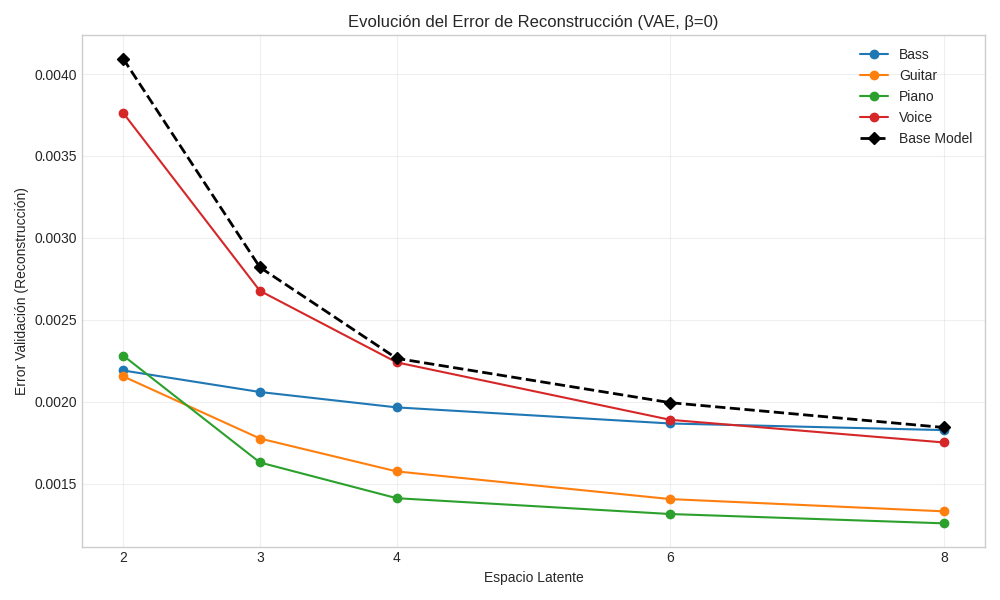
\includegraphics[scale=0.45]{imgs/01_arquitectura/5_recon_evolution_no_beta.png}
\end{figure}

Analizando los resultados de las figuras~\ref{fig:mse_vs_dim} y~\ref{fig:mse_vs_dim_prom} observamos que, con un espacio latente de dimensión $4$, obtenemos una ganancia significativa respecto a las dimensiones $2$ y $3$, mientras que aumentar el tamaño a $6$ u $8$ no aporta una mejora relevante.

Nos interesa también verificar este comportamiento para la arquitectura $\beta$-VAE, donde esperamos observar un error de reconstrucción mayor en magnitud---ya que la \textit{loss} de estos modelos incorpora también la divergencia KL---pero con la misma tendencia.


\begin{figure}[H]
\caption{Error de Reconstrucción promedio general}
\centering
\label{fig:mse_vs_dim_prom}
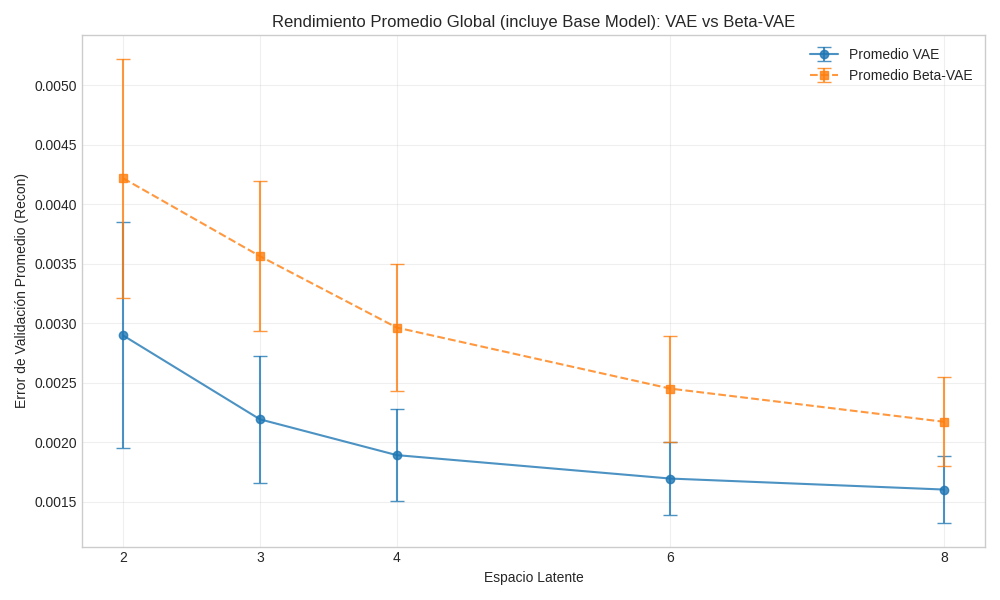
\includegraphics[scale=0.45]{imgs/01_arquitectura/2_val_loss_mean_std_with_base.png}
\end{figure}

En efecto, lo observado para los modelos AE (con $\beta=0$) se cumple también con $\beta$ activado. Resta verificar el comportamiento de la divergencia KL en los modelos $\beta$-VAE para los distintos tamaños de espacio latente, presentado en la figura~\ref{fig:kl_vs_dim}.

\begin{figure}[H]
\caption{Divergencia KL vs Dimensión de espacio latente, $\beta=0.001$}
\centering
\label{fig:kl_vs_dim}
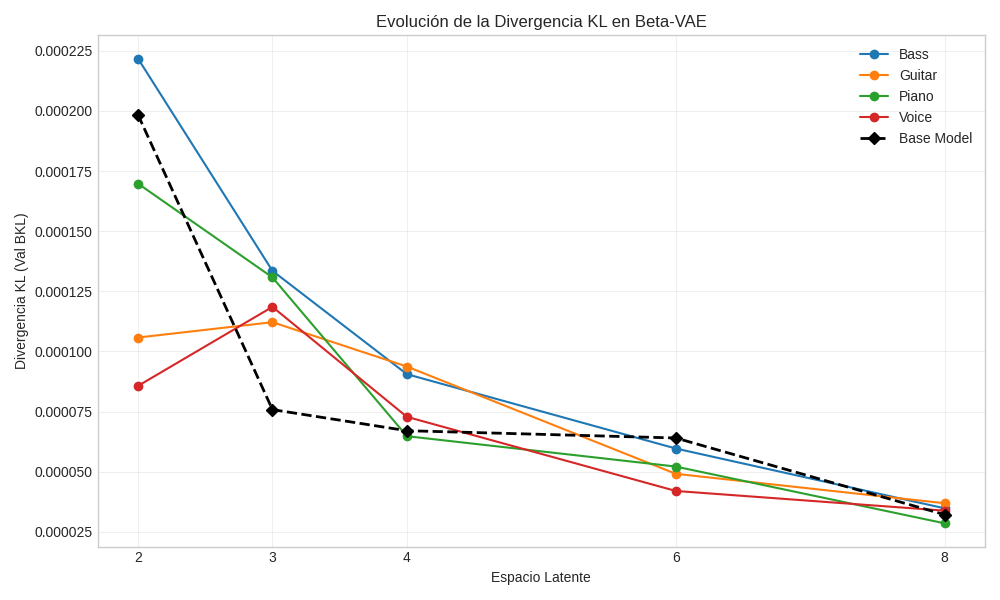
\includegraphics[scale=0.45]{imgs/01_arquitectura/4_beta_kl_evolution.png}
\end{figure}

Efectivamente, el salto más significativo se encuentra entre las dimensiones $2$ y $4$, y a partir de allí la KL sigue disminuyendo pero con una ganancia relativa menor. En la figura~\ref{fig:mse_per_instrument} se presenta además el desglose del error de reconstrucción por instrumento, que confirma la misma tendencia. En base a estos resultados, adoptamos para el resto de los experimentos arquitecturas con espacio latente de dimensión $4$.

\begin{figure}[H]
\caption{Desglose: Error de Reconstrucción (MSE) por modelo}
\centering
\label{fig:mse_per_instrument}
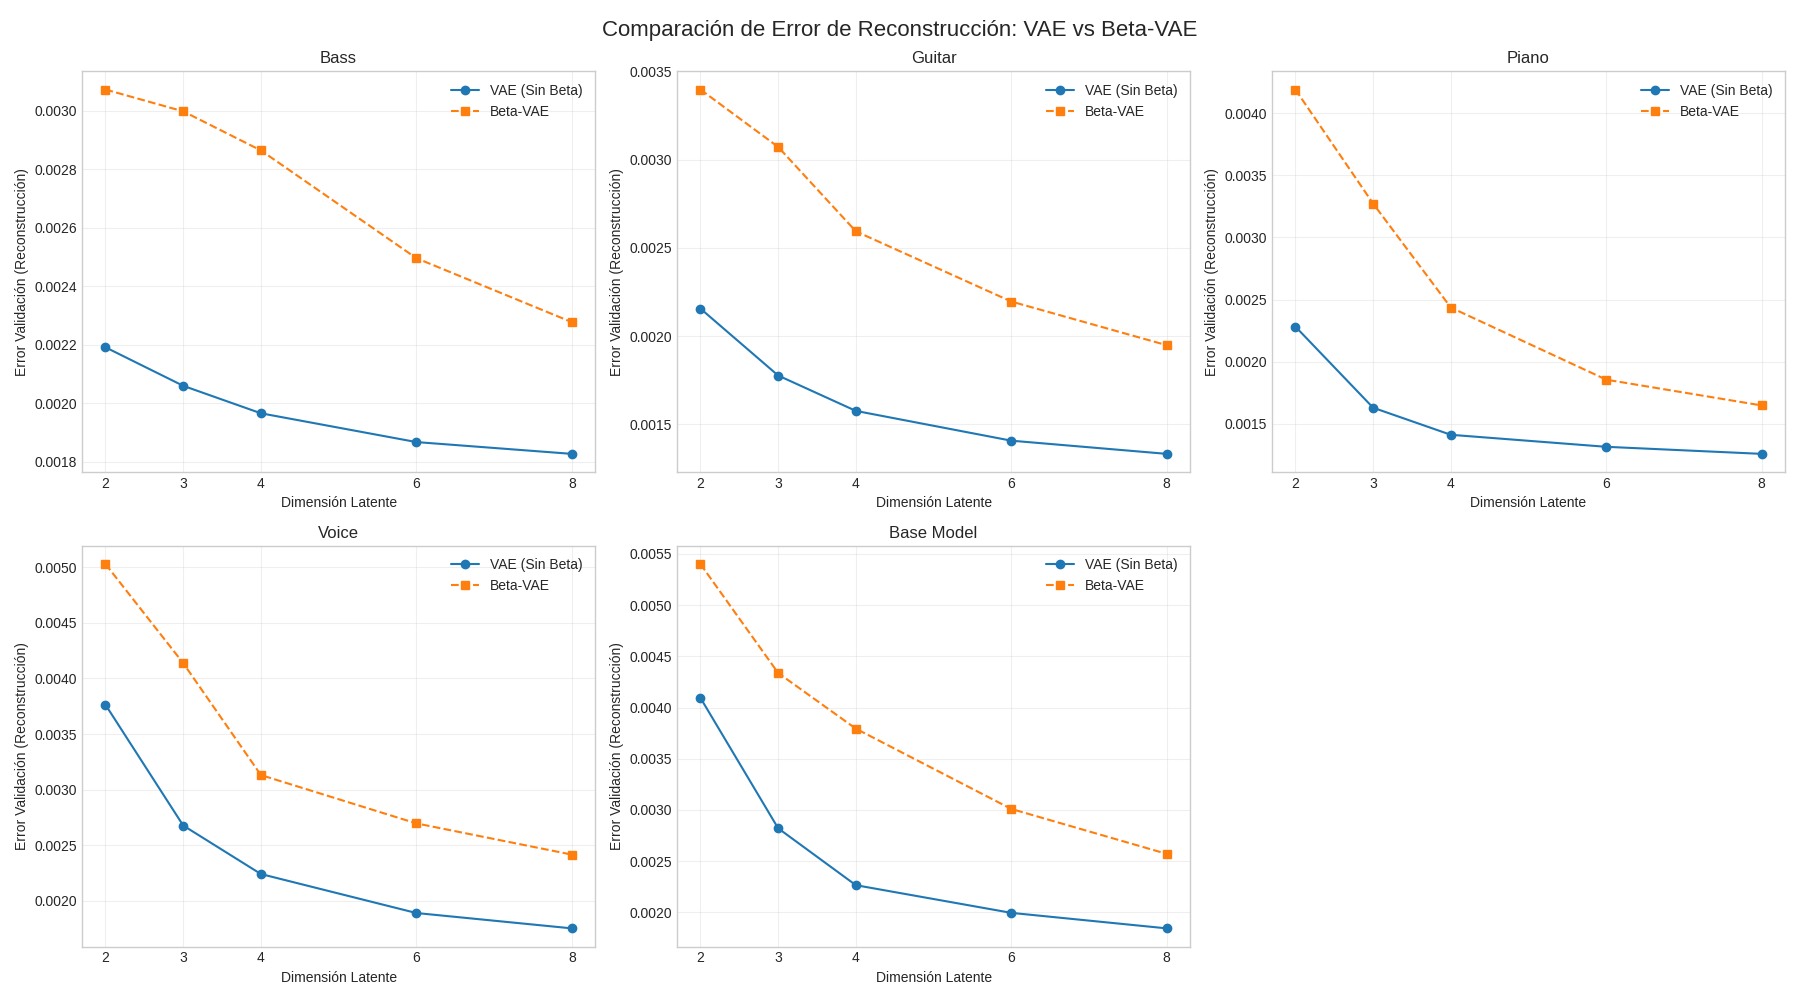
\includegraphics[scale=0.35]{imgs/01_arquitectura/1_comparacion_por_instrumento.png}
\end{figure}

\begin{comment}
    
\section{Entrenamiento}

Queremos validar que 

\begin{figure}[H]
\caption{Evolución de error de reconstrucción durante entrenamiento}
\centering
\label{fig:centralidad}
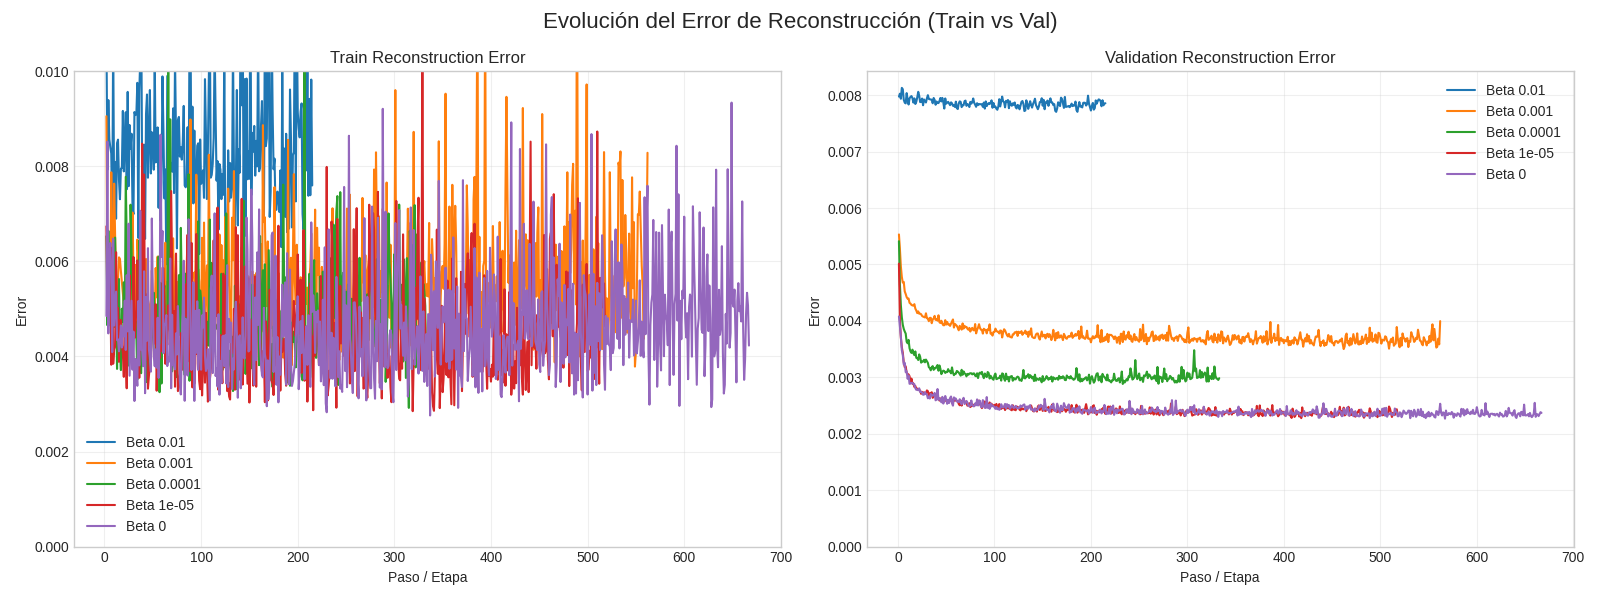
\includegraphics[scale=0.375]{imgs/02_comparacion_beta_vae/recon_evolution.png}
\end{figure}

\begin{figure}[H]
\caption{Evolución divergencia KL durante entrenamiento}
\centering
\label{fig:centralidad}
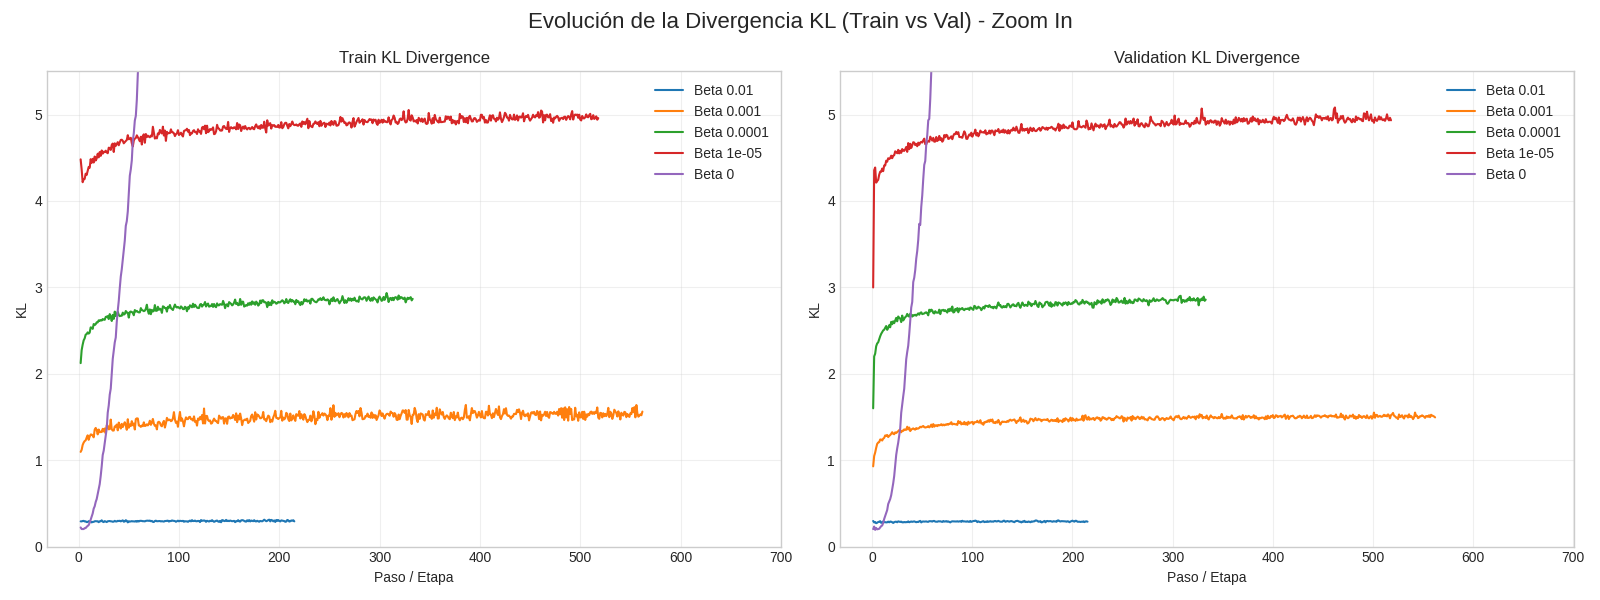
\includegraphics[scale=0.375]{imgs/02_comparacion_beta_vae/kl_evolution_0.002.png}
\end{figure}

\begin{figure}[H]
\caption{Evolución Divergecia KL, Zoom Out:}
\centering
\label{fig:centralidad}
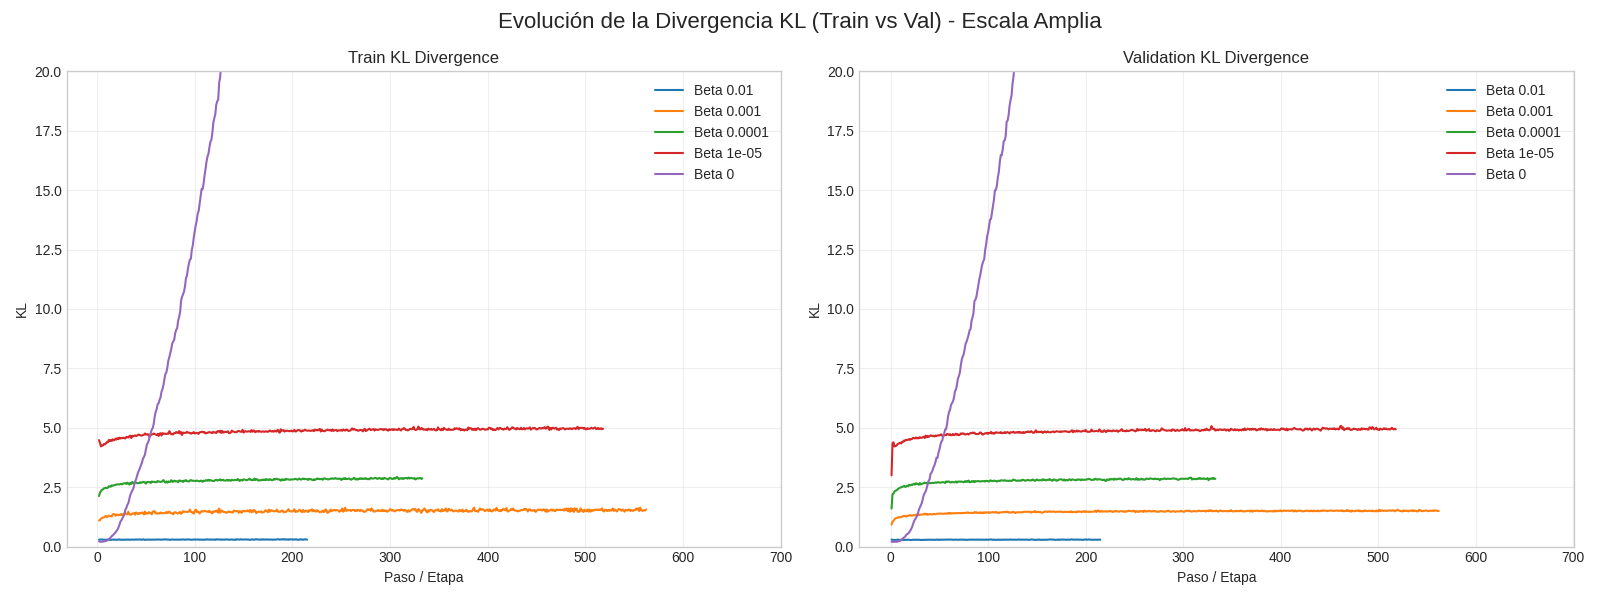
\includegraphics[scale=0.375]{imgs/02_comparacion_beta_vae/kl_evolution_0.2.png}
\end{figure}
\end{comment}

\section{Análisis del Espacio Latente}

Para analizar la organización del espacio latente del modelo base, proyectamos los \textit{embeddings} a $2$ dimensiones mediante UMAP, etiquetando cada muestra con el instrumento al que corresponde. Esto nos permite evaluar visualmente si los distintos instrumentos forman \textit{clusters} diferenciados y comparar el comportamiento entre las configuraciones $\beta=0$ y $\beta=0.001$. Los resultados se presentan en la figura~\ref{fig:umap}.

\begin{figure}[H]
\caption{Proyección a 2 dimensiones del espacio latente del modelo base utilizando UMAP.}
\label{fig:umap}
\begin{subfigure}{.5\textwidth}
    \caption{$\beta = 0.001$.}
    \centering
    \label{fig:umap_beta}
    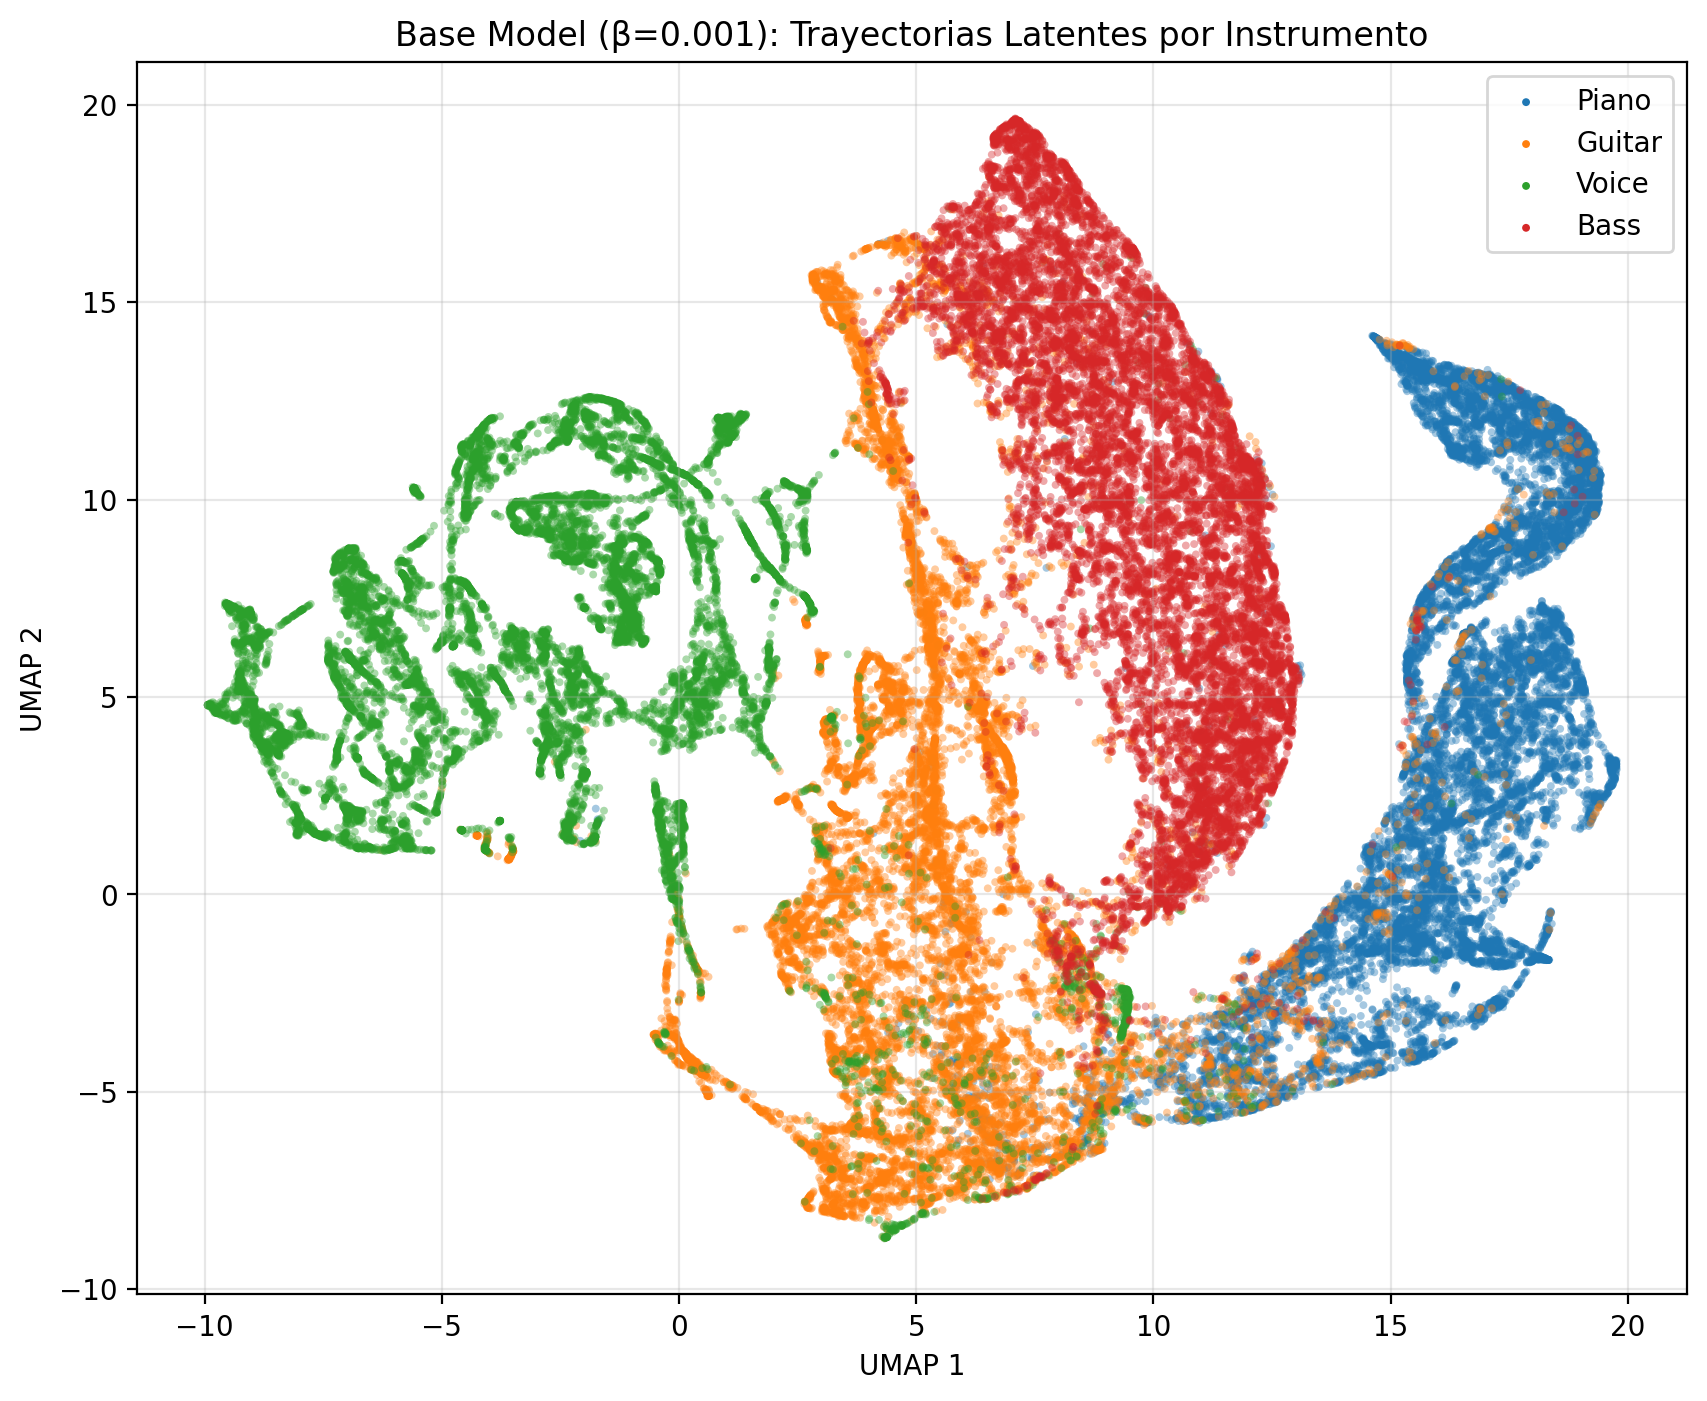
\includegraphics[width=\linewidth]{imgs/03_umap/base_model_beta_instruments_umap.png}
\end{subfigure}
\begin{subfigure}{.5\textwidth}
    \caption{$\beta=0$.}
    \centering
    \label{fig:umap_no_beta}
    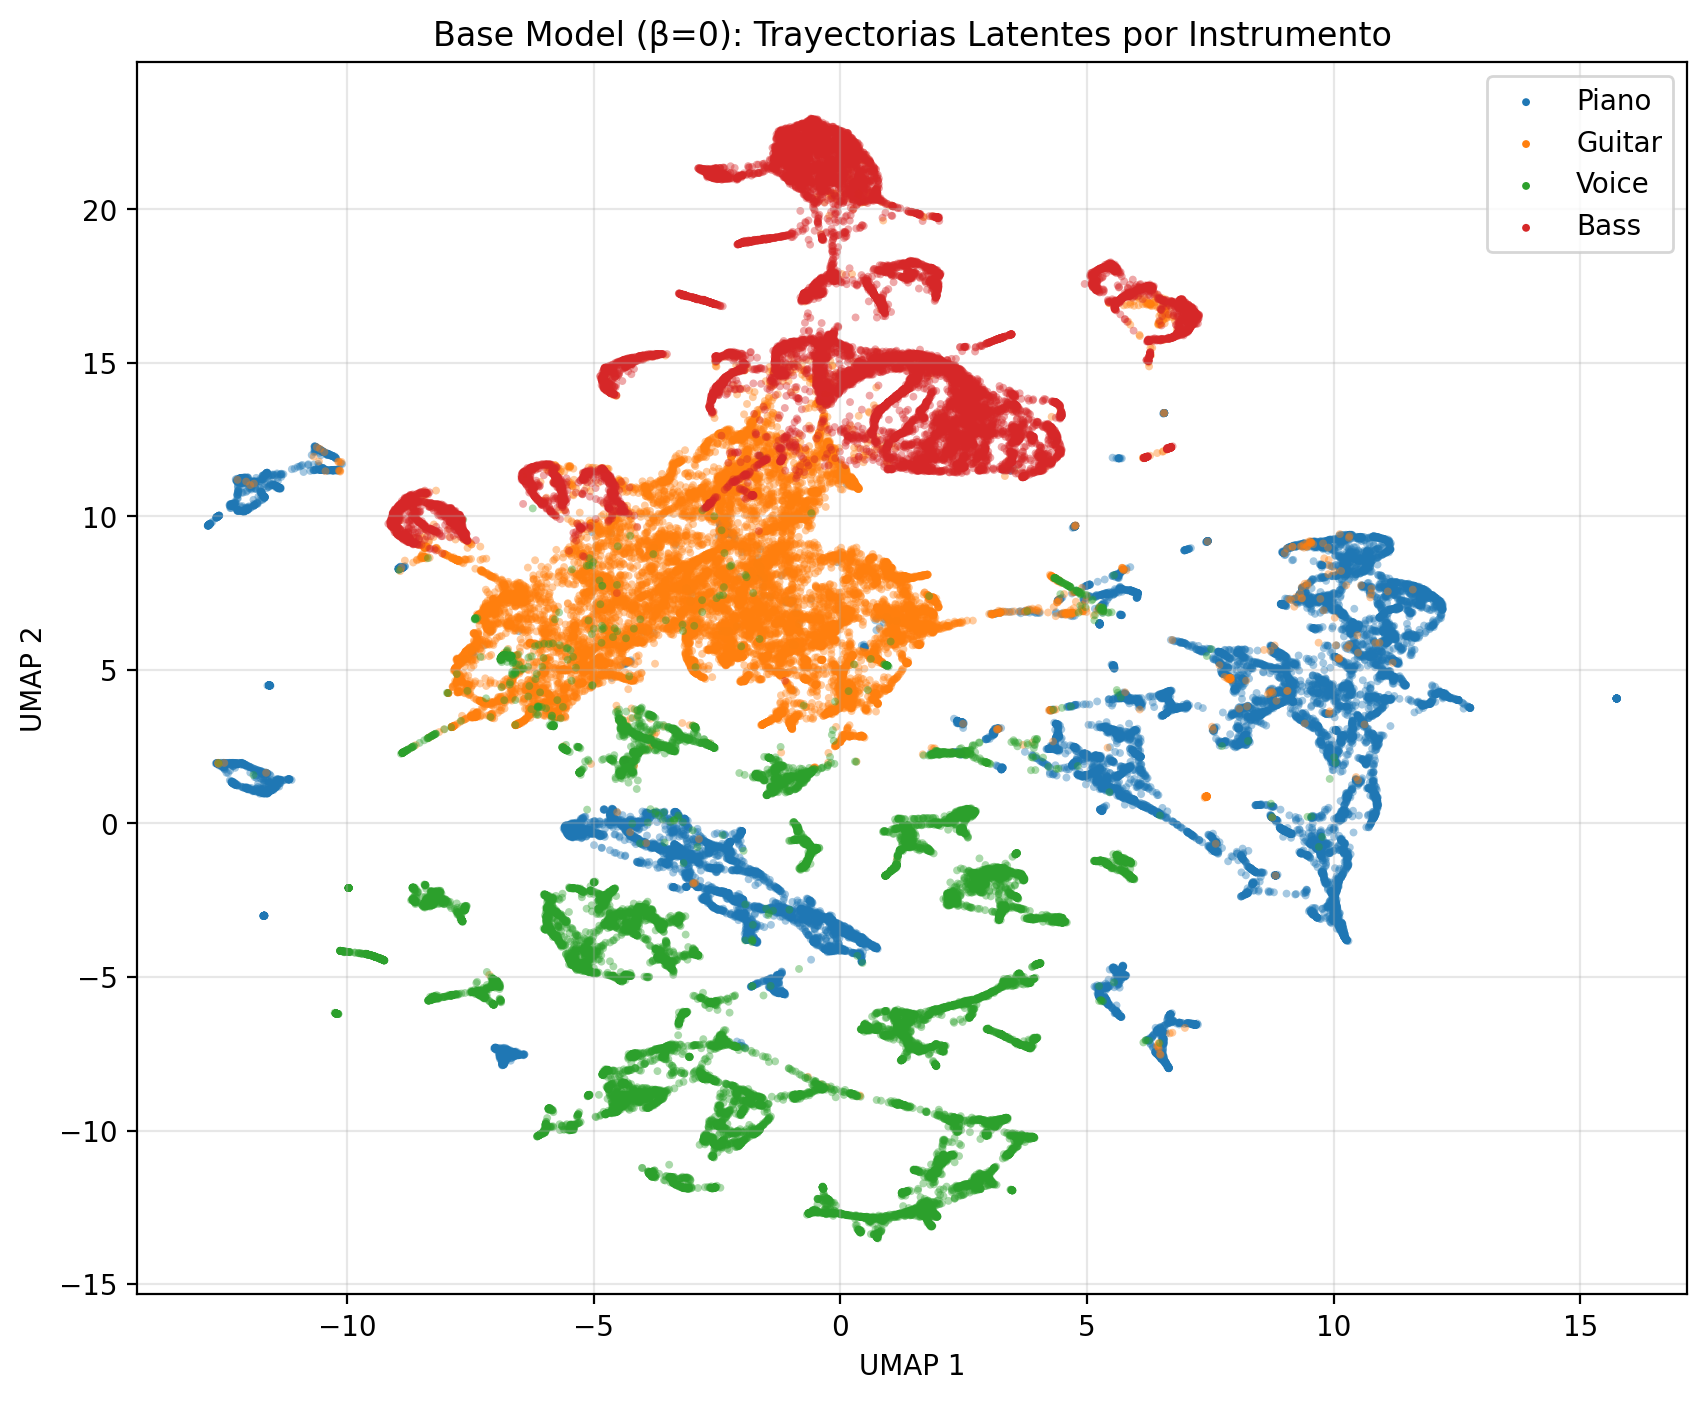
\includegraphics[width=\linewidth]{imgs/03_umap/base_model_no_beta_instruments_umap.png}
\end{subfigure}
\end{figure}

Para cuantificar la separación entre los \textit{clusters} de cada instrumento computamos las distancias entre sus centroides en la proyección UMAP, sintetizadas en la matriz de la figura~\ref{fig:umap_sep}.

\begin{figure}[H]
\caption{Matriz de separación entre \textit{clusters} de instrumentos en la proyección UMAP.}
\label{fig:umap_sep}
\begin{subfigure}{.5\textwidth}
    \caption{$\beta = 0.001$.}
    \centering
    \label{fig:umap_sep_beta}
    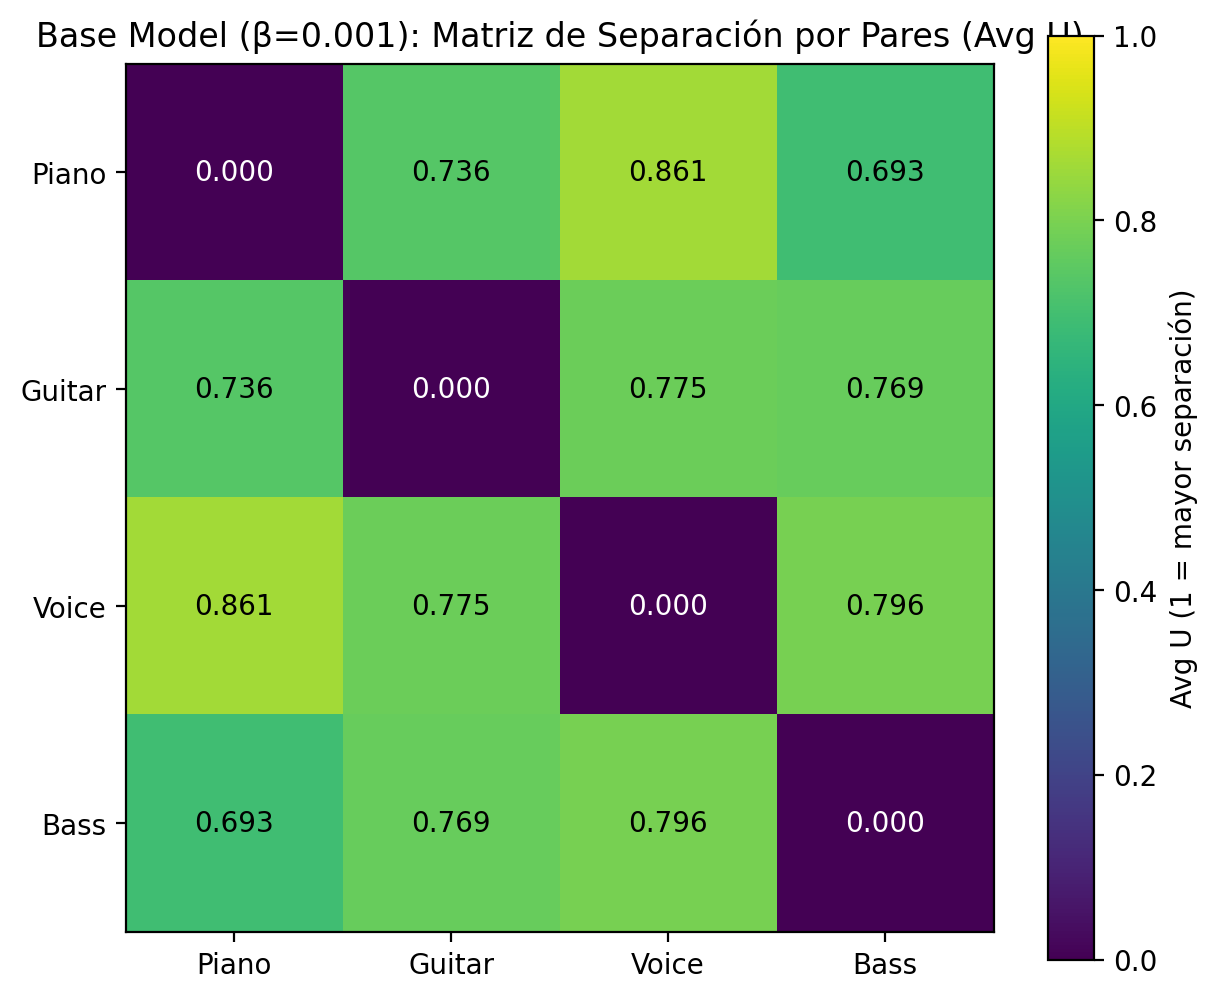
\includegraphics[width=\linewidth]{imgs/03_umap/base_model_beta_instruments_umap_separation_matrix.png}
\end{subfigure}
\begin{subfigure}{.5\textwidth}
    \caption{$\beta = 0$.}
    \centering
    \label{fig:umap_sep_no_beta}
    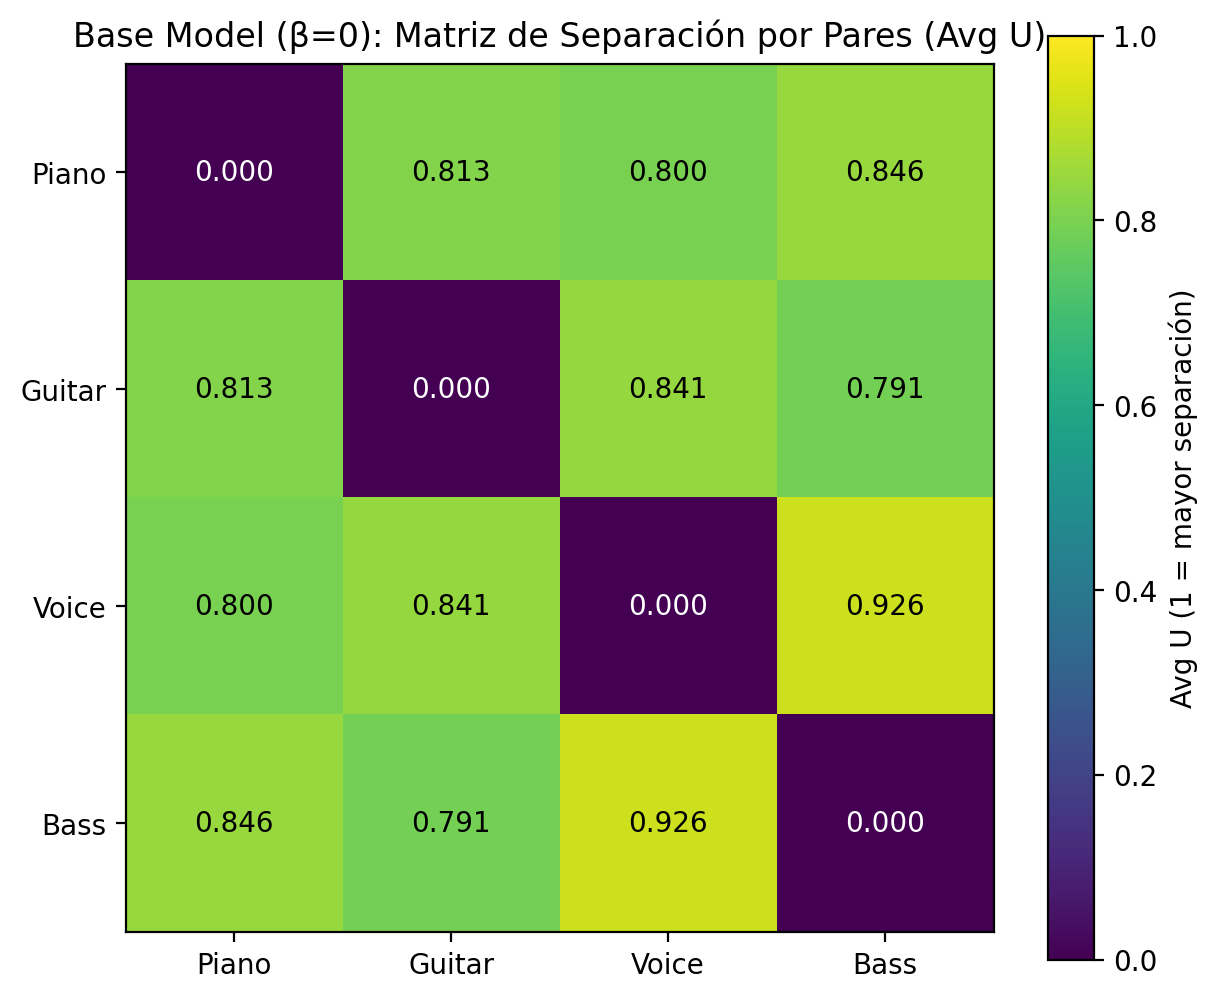
\includegraphics[width=\linewidth]{imgs/03_umap/base_model_no_beta_instruments_umap_separation_matrix.png}
\end{subfigure}
\end{figure}


\section{Interpolación}

Esta sección se centra en la interpolación de pesos entre dos modelos especializados en instrumentos distintos. Tal como se definió en la sección de metodología, generaremos un modelo intermedio en función de tres parámetros: un modelo origen A, un modelo destino B y un coeficiente de interpolación $\alpha \in [0, 1]$. De este modo, con $\alpha=0$ obtenemos exactamente el modelo A, y con $\alpha=1$ obtenemos el modelo B. 

El objetivo principal de esta interpolación es lograr una transferencia tímbrica suave entre ambos modelos. Por ejemplo, si establecemos un modelo de voz como modelo A y un modelo de piano como modelo B, el comportamiento esperado es que, a medida que $\alpha$ se incrementa de $0$ a $1$, el audio sintetizado adquiera progresivamente características tímbricas más cercanas a las del piano.

A lo largo de los experimentos, analizaremos el impacto de las distintas configuraciones de entrenamiento introducidas previamente. Para mantener la consistencia, clasificaremos los modelos según su inicialización: desde cero (\textit{Scratch}) o desde un modelo base pre-entrenado (\textit{Checkpoint}); y según su regularización en el espacio latente: Autoencoder estándar (AE, con $\beta=0$) o $\beta$-VAE (con $\beta=0.001$).

\subsection{Elección de Métricas de Similitud}

Para evaluar empíricamente la interpolación, resulta indispensable definir una métrica que cuantifique la similitud tímbrica entre la salida de los modelos y los audios de referencia. En este trabajo, comparamos el desempeño de dos enfoques: la similitud coseno entre embeddings extraídos con MERT, y la Distancia de Fréchet para Audio (FAD, por sus siglas en inglés) \cite{gui2024adaptingfrechetaudiodistance}, la cual es altamente citada en la literatura sobre el tema.

La principal diferencia teórica entre ambas recae en que FAD considera la varianza de las distribuciones, lo que a priori mejoraría su precisión al evaluar fragmentos de audio de mayor duración. Sin embargo, en instantes de audio cortos (pocos frames de sonido constante) donde prima el análisis tímbrico, ambas métricas deberían ofrecer resultados comparables.

Para validar esto empíricamente, evaluamos la interpolación de voz a piano utilizando como referencia el audio reconstruido por el modelo de piano. Analizamos dos escenarios de entrada para el decoder: partiendo de un vector latente $Z$ aleatorio fijo, y partiendo de un vector latente $Z$ proveniente de codificar un fragmento de audio de validación. Comparamos los resultados utilizando dos configuraciones extremas: \textit{Scratch-AE} ($\beta=0$) y \textit{Checkpoint-$\beta$-VAE} ($\beta=0.001$).

\begin{figure}[H]
\caption{Comparación de métricas (Similitud Coseno vs. FAD) partiendo de un vector latente $Z$ aleatorio.}
\label{fig:cos_fad_zrandom}
\begin{subfigure}{.5\textwidth}
\caption{Configuración: \textit{Scratch-AE} ($\beta = 0$).}
\centering
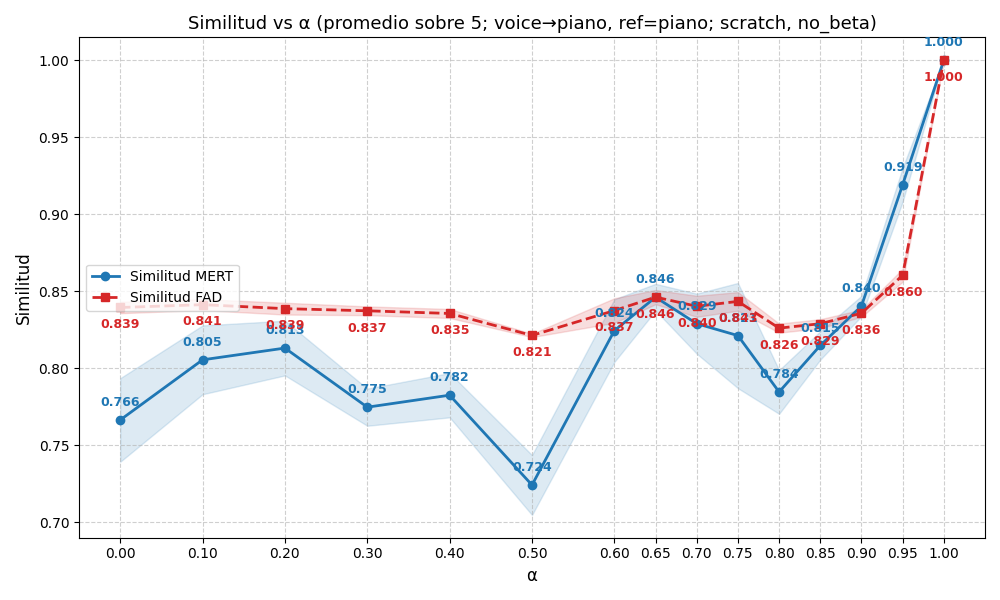
\includegraphics[width=\linewidth]{imgs/04_similitud/sim_scratch_no_beta_zrandom.png}
\end{subfigure}
\begin{subfigure}{.5\textwidth}
\caption{Configuración: \textit{Checkpoint-$\beta$-VAE} ($\beta = 0.001$).}
\centering
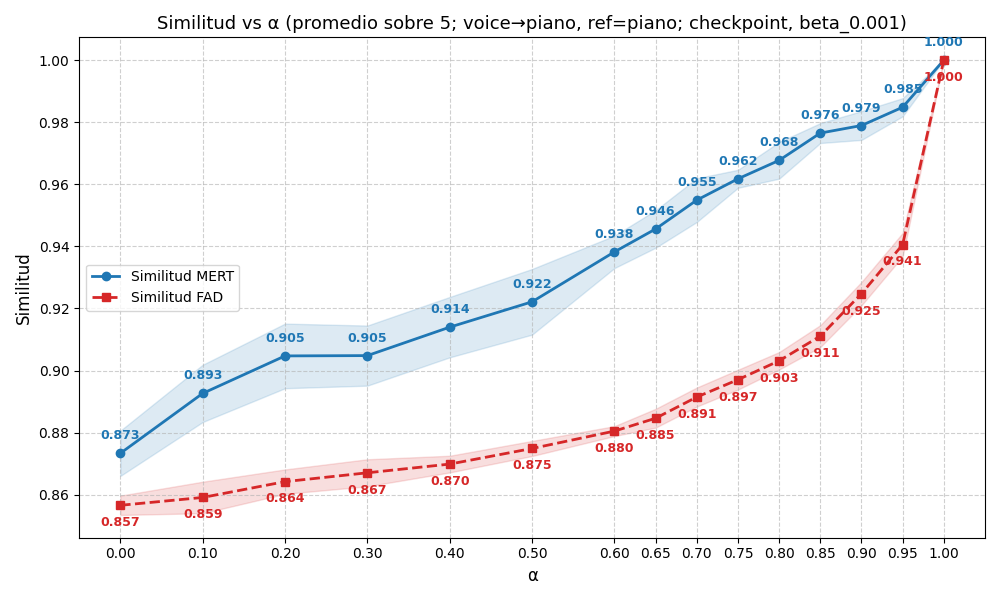
\includegraphics[width=\linewidth]{imgs/04_similitud/sim_checkpoint_beta_zrandom.png}
\end{subfigure}
\end{figure}

Los resultados presentados en la Figura \ref{fig:cos_fad_zrandom} ilustran el comportamiento partiendo de un $Z$ aleatorio. Para la configuración \textit{Scratch-AE}, es esperable que no haya una transición suave (ya que interpolamos espacios latentes disjuntos y sin regularizar); no obstante, se observa que la similitud coseno presenta picos y fluctuaciones erráticas, mientras que FAD se mantiene notablemente más estable. Por el contrario, en la configuración \textit{Checkpoint-$\beta$-VAE}, ambas métricas muestran el crecimiento suave y sostenido esperado, presentando una alta correlación en este escenario estático.

\begin{figure}[H]
\caption{Comparación de métricas (Similitud Coseno vs. FAD) partiendo de un vector latente $Z$ codificado desde un audio real.}
\label{fig:cos_fad_zencoded}
\begin{subfigure}{.5\textwidth}
\caption{Configuración: \textit{Scratch-AE} ($\beta = 0$).}
\centering
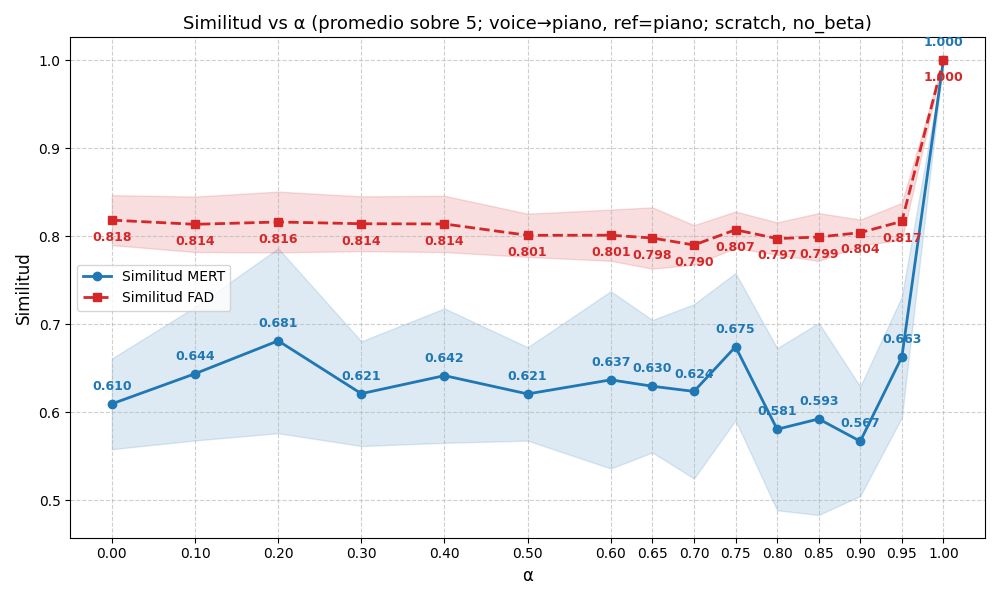
\includegraphics[width=\linewidth]{imgs/04_similitud/sim_scratch_no_beta_zencoded.png}
\end{subfigure}
\begin{subfigure}{.5\textwidth}
\caption{Configuración: \textit{Checkpoint-$\beta$-VAE} ($\beta = 0.001$).}
\centering
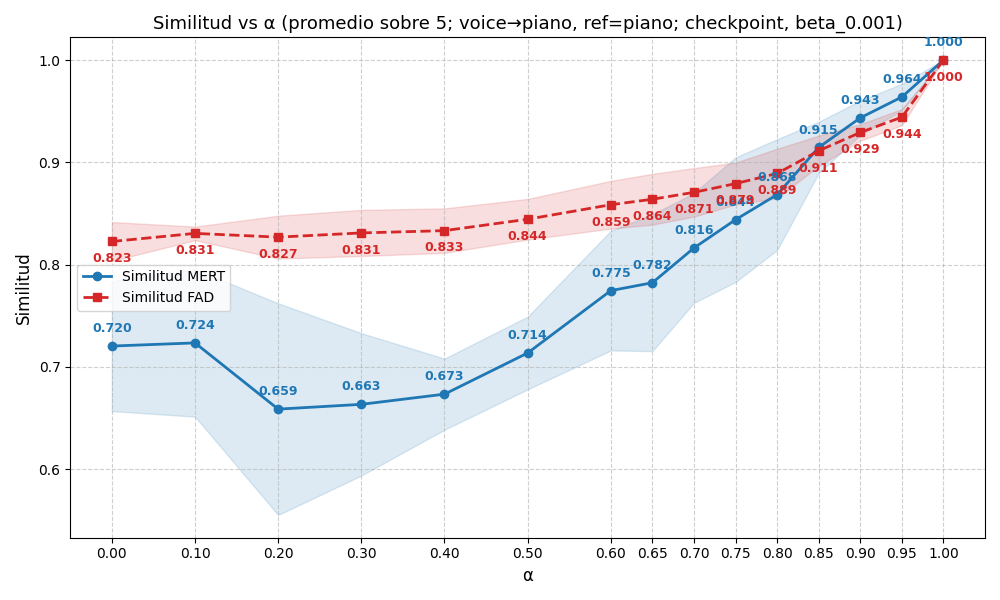
\includegraphics[width=\linewidth]{imgs/04_similitud/sim_checkpoint_beta_zencoded.png}
\end{subfigure}
\end{figure}

Al evaluar con un vector latente $Z$ proveniente de un audio real (Figura \ref{fig:cos_fad_zencoded}), las deficiencias de la similitud coseno se hacen más evidentes. En la configuración \textit{Scratch-AE}, la similitud coseno sufre una alta variación y dispersión. FAD, en cambio, captura correctamente que el modelo no logra asimilarse al timbre destino hasta llegar a $\alpha \approx 0.95$.

En la configuración \textit{Checkpoint-$\beta$-VAE}, FAD traza una curva de crecimiento predecible y suave con baja desviación estándar, confirmando que la interpolación es efectiva. La similitud coseno, aunque logra marcar la tendencia general de transferencia tímbrica, presenta caídas anómalas (e.g., en $\alpha=0.20$) y mayor dispersión. Dado que FAD demostró ser más robusta y consistente frente a distintas entradas y configuraciones, nos basaremos en ella para el resto de los experimentos de esta sección.

\subsection{Experimentos de Interpolación}

Habiendo validado la métrica, procedemos a verificar si la transferencia tímbrica hacia un instrumento de destino (piano) se sostiene independientemente del instrumento de origen (bajo, guitarra, voz). Evaluamos múltiples muestras de vectores $Z$ para cada caso y graficamos el promedio de la similitud FAD junto con su dispersión.

\begin{figure}[H]
\caption{Comparación agregada entre configuraciones, interpolando desde múltiples instrumentos hacia piano.}
\centering
\label{fig:sim_aggregated}
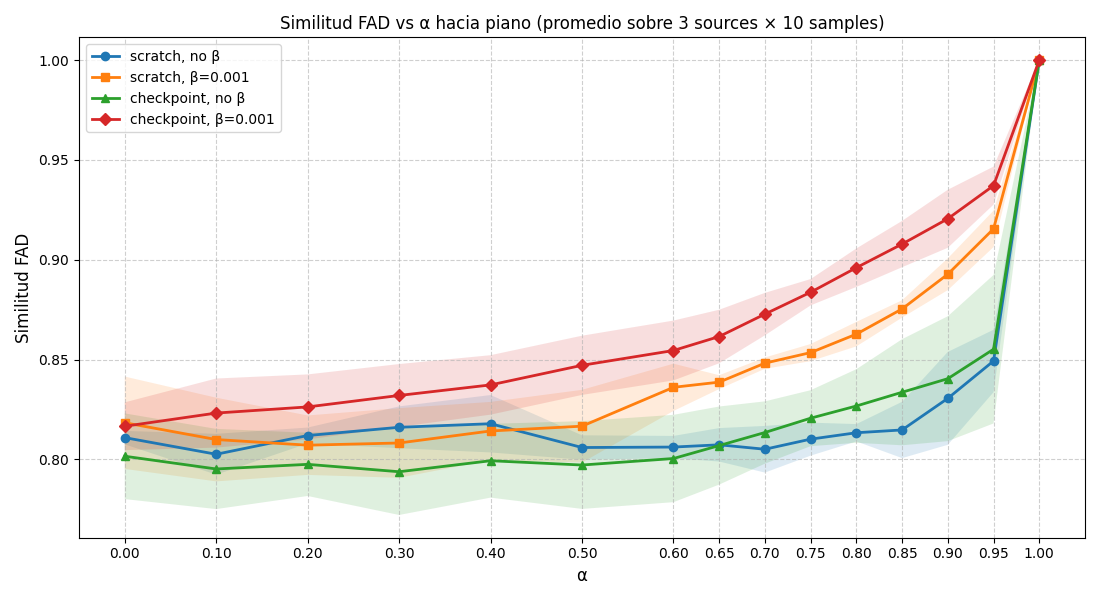
\includegraphics[scale=0.5]{imgs/04_similitud/sim_aggregated_to_piano.png}
\end{figure}

Como se observa en la Figura \ref{fig:sim_aggregated}, existe una transferencia tímbrica en todos los escenarios, pero las diferencias de rendimiento entre configuraciones son notables. La curva de mejor comportamiento corresponde a \textit{Checkpoint-$\beta$-VAE} ($\beta=0.001$), seguida por \textit{Scratch-$\beta$-VAE}. Esto sugiere fuertemente que la regularización impuesta por $\beta>0$ para suavizar el espacio latente es el factor de mayor impacto para lograr interpolaciones de alta calidad. Secundariamente, compartir un punto de partida común en los pesos del modelo (\textit{Checkpoint}) aporta una mejora adicional frente a los modelos entrenados desde cero.

\begin{figure}[H]
\caption{Desglose por instrumento de origen para la configuración \textit{Checkpoint-$\beta$-VAE} ($\beta=0.001$).}
\centering
\label{fig:sim_aggregated_per_instrument_checkpoint}
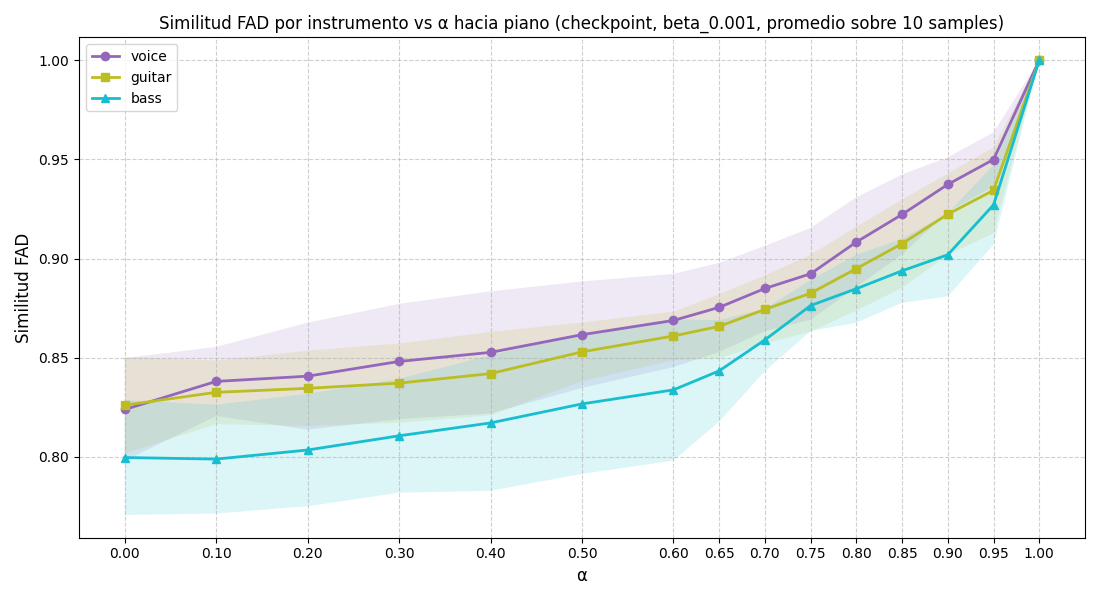
\includegraphics[scale=0.5]{imgs/04_similitud/desglose_aggregated_checkpoint_beta.png}
\end{figure}
\begin{figure}[H]
\caption{Desglose por instrumento de origen para la configuración \textit{Scratch-AE} ($\beta=0$).}
\centering
\label{fig:sim_aggregated_per_instrument_scratch}
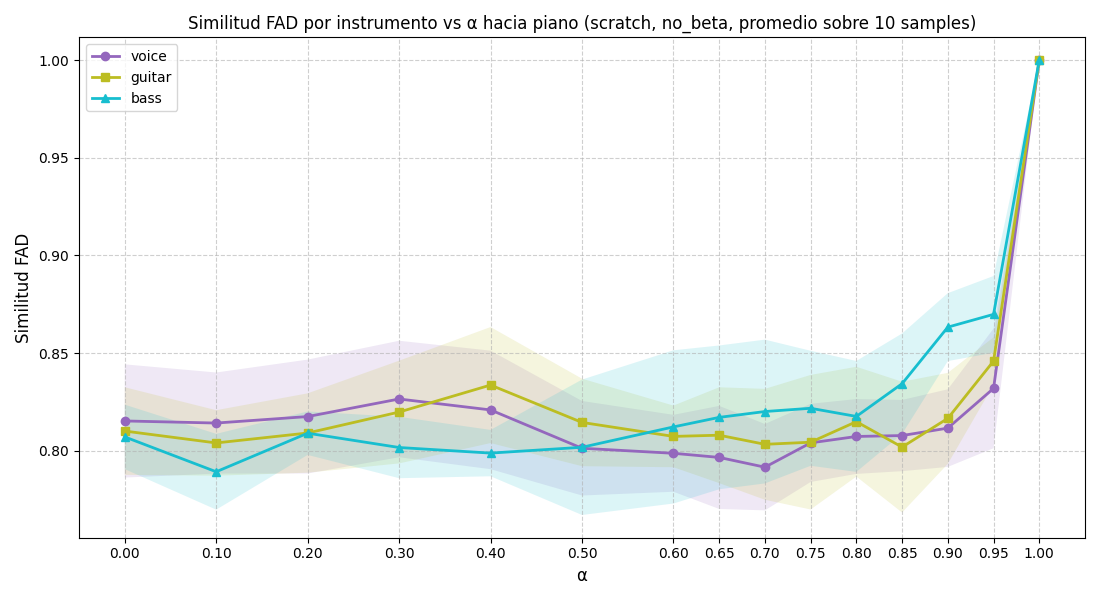
\includegraphics[scale=0.5]{imgs/04_similitud/desglose_aggregated_scratch_no_beta.png}
\end{figure}

Al desglosar los resultados (Figuras \ref{fig:sim_aggregated_per_instrument_checkpoint} y \ref{fig:sim_aggregated_per_instrument_scratch}), confirmamos que este patrón es consistente para cualquier instrumento de origen. Queda en evidencia que los modelos sin regularizar (\textit{Scratch-AE}) fracasan en realizar una transición gradual, retrasando el cambio tímbrico hacia los valores extremos de $\alpha$.

TODO: Ahora repetimos este análisis usando cada posible instrumento como destino, y en cada caso los otros 3 instrumentos como origen. Tomamos el promedio y obtuvimos el siguiente gráfico:

\begin{figure}[H]
\caption{Comparación agregada entre configuraciones, interpolando desde múltiples instrumentos hacia todos los instrumentos.}
\centering
\label{fig:sim_aggregated_all_instruments}
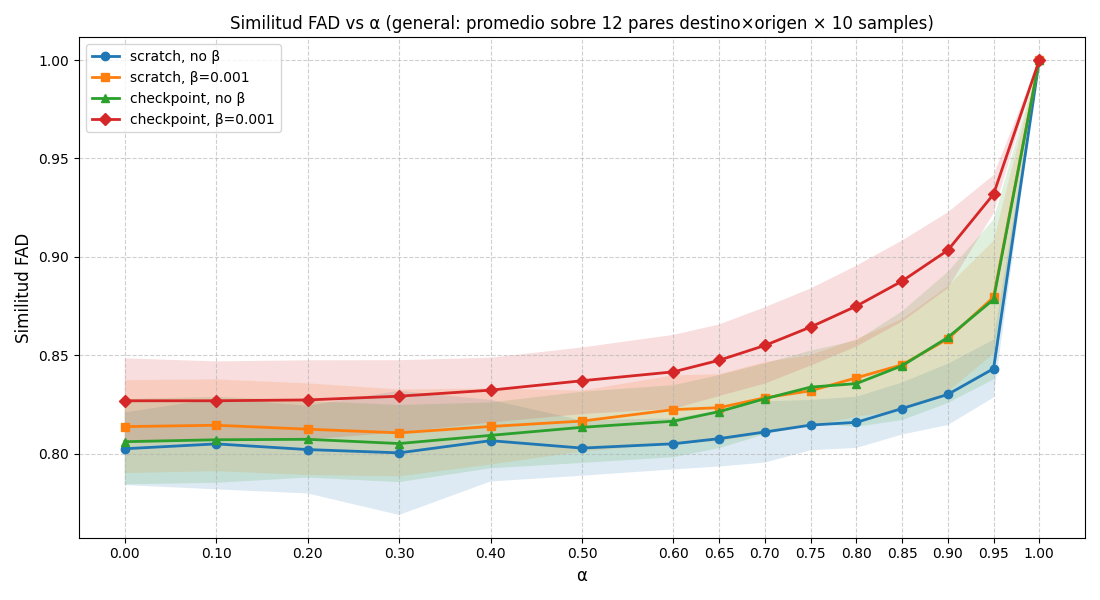
\includegraphics[scale=0.5]{imgs/04_similitud/sim_aggregated_to_all_instruments.png}
\end{figure}

TODO: Análisis: se observa claramente a lo largo de los diferentes samples y las diferentes combinaciones de instrumentos de origen y destino que la mejor configuración es la checkpoint beta. Luego, tanto agregar sólo beta como agregar sólo checkpoint genera una mejora en la similitud en comparación con el peor enfoque que es scratch no beta. Esto es consistente a lo largo de todas las pruebas de combinaciones de instrumentos como origen/destino.



Para dar el análisis por concluido, resta verificar una última condición: a medida que el audio sintetizado se aproxima tímbricamente al instrumento B, debe necesariamente alejarse de las características del instrumento A, y, fundamentalmente, no debe adoptar rasgos de otros instrumentos ajenos a la interpolación (un instrumento \textit{testigo}).

Se espera que, a medida que $\alpha$ crezca, la similitud con el instrumento B aumente y la del instrumento A disminuya, cruzándose aproximadamente en $\alpha=0.5$. Simultáneamente, la similitud con el instrumento testigo debería mantenerse constante. Para este experimento definimos piano como instrumento A, guitarra como instrumento B, y voz como instrumento testigo.

\begin{figure}[H]
\caption{Transición cruzada de piano a guitarra. Comparación entre orígenes (\textit{Checkpoint} vs. \textit{Scratch}) y regularización ($\beta$). La voz actúa como instrumento testigo.}
\centering
\label{fig:transicion_piano_guitarra}
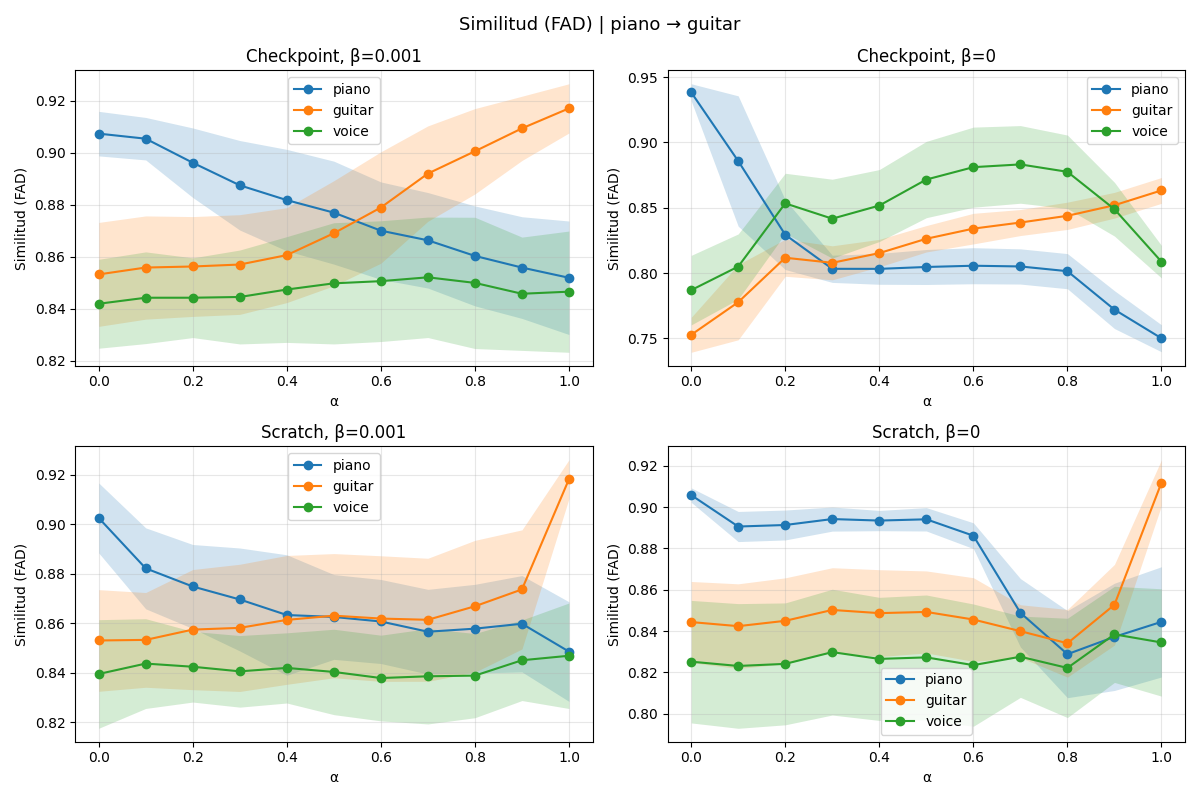
\includegraphics[scale=0.5]{imgs/plots/fad_random_latent_gaussian_piano_to_guitar.png}
\end{figure}

Los resultados presentados en la Figura \ref{fig:transicion_piano_guitarra} corroboran nuestra hipótesis para la configuración \textit{Checkpoint-$\beta$-VAE}. Se observa que la similitud con el piano decrece de manera consistente mientras la similitud con la guitarra aumenta, ocurriendo el punto de cruce alrededor de $\alpha=0.5$, todo esto mientras la voz (instrumento testigo) se mantiene constante.

Por el contrario, los modelos entrenados desde \textit{Scratch} exhiben un comportamiento indeseable. Aún con $\beta=0.001$, la transferencia es poco consistente para valores intermedios de $\alpha$; y con $\beta=0$, la transición es prácticamente inexistente hasta $\alpha>0.8$. El caso de \textit{Checkpoint-AE} ($\beta=0$) logra la transferencia deseada, pero de forma mucho más abrupta, provocando además fluctuaciones erráticas en la curva del instrumento testigo.

En conclusión, estos experimentos confirman empíricamente que la arquitectura más robusta para garantizar una transferencia tímbrica predecible, gradual e independiente en la interpolación de pesos es la basada en modelos con inicialización común y espacios latentes regularizados (\textit{Checkpoint} con $\beta=0.001$).

\begin{comment}
    
\section{Barrido de dimensión del espacio latente}
% Dims (2,3,4,6,8) × instrumento × 5 repeticiones, VAE vs β-VAE.

\section{Variación de $\beta$}
% β ∈ {0, 1e-5, 1e-4, 1e-3, 1e-2} sobre el modelo base. Evolución del MSE
% y KL durante el entrenamiento.

\section{Análisis del espacio latente con UMAP}
% Proyección 2D del espacio latente del modelo base; clustering por
% instrumento; U de Wilcoxon-Mann-Whitney multidimensional.

\section{Interpolación entre pares de instrumentos}
% Similitud de reconstrucción vs α para los 6 pares; comparación
% from-checkpoint vs from-scratch y β vs no-β.

\section{Audio morphing}
% Transiciones audio-a-audio encodeando muestras reales, blending
% secuencial de Z e interpolación de pesos.
\end{comment}


\chapter{Conclusiones}
\label{cap:conclusiones}

\section{Resumen de resultados}

\section{Contribuciones}

\section{Limitaciones}

\section{Trabajo futuro}


%%%% BIBLIOGRAFIA
\backmatter
\bibliographystyle{acm}
\bibliography{bibliografia}

\end{document}
